\documentclass[t,xcolor=table,usenames,dvipsnames]{beamer}
%\documentclass[handout,t,xcolor=table,usenames,dvipsnames]{beamer}

\usepackage[SlantFont, BoldFont]{xeCJK}

\usepackage{fontspec}
\linespread{1.24}
\setmainfont[Mapping=tex-text,LetterSpace=-1.0]{DejaVu Sans}
\setsansfont[Mapping=tex-text,LetterSpace=-1.0]{DejaVu Sans}
\setmonofont[Color=00663300]{DejaVu Sans Mono}
\setCJKmainfont[Scale=1.2,BoldFeatures={FakeBold=3}]{cwTeX Q Hei Bold}
\setCJKmonofont[Scale=1.2,BoldFeatures={FakeBold=4},FakeStretch=1.01532,Color=00663300]{cwTeX Q Yuan}

\XeTeXlinebreaklocale "zh"
\XeTeXlinebreakskip = 0pt plus 1pt

% Show current position in each slide
%\useoutertheme{shadow}
%\useoutertheme{tree}
\useinnertheme[shadow=true]{rounded}

% item icon: default, ball, circle, rectangle
\setbeamertemplate{items}[rectangle]

% numbering figure and table
\setbeamertemplate{caption}[numbered]

% dove, spruce, beaver, seahorse
\usecolortheme{spruce}

% chapter list
\setbeamercolor*{palette quaternary}{fg=black,bg=MSUgreen!35!white}
% block
\setbeamercolor{block title}{use=structure,fg=white,bg=MSUgreen!75!black}


% reset footline
\setbeamertemplate{footline}
{
\leavevmode
\hbox{
    \begin{beamercolorbox}[wd=.163\paperwidth,ht=2.25ex,dp=1ex,center]{author in head/foot}
        \usebeamerfont{author in head/foot}\insertshortauthor
    \end{beamercolorbox}
%
    \begin{beamercolorbox}[wd=.823\paperwidth,ht=2.25ex,dp=1ex,center]{title in head/foot}
        \usebeamerfont{title in head/foot}\insertshorttitle\hspace*{3em}
%    \end{beamercolorbox}
%
%    \begin{beamercolorbox}[wd=.303\paperwidth,ht=2.25ex,dp=1ex,right]{date in head/foot}
%        \usebeamerfont{date in head/foot}\insertshortdate{}\hspace*{2em}
        \insertframenumber{} / \inserttotalframenumber\hspace*{1em}
    \end{beamercolorbox}
        }
\vskip0pt
}

% remove right-bottom navigation
\setbeamertemplate{navigation symbols}{}
% use default bullet style: http://tex.stackexchange.com/questions/11168/change-bullet-style-formatting-in-beamer
\setbeamertemplate{itemize items}[default]
\setbeamertemplate{enumerate items}[default]
\setbeamercolor{local structure}{fg=MSUgreen}

%\usepackage{hyperref,url}
%\usepackage[none]{hyphenat}
%\usepackage[bottom]{footmisc}

\usepackage{color}
%\usepackage{xcolor}
\usepackage{tabularx}

\usepackage{listings}

%\usepackage{caption}
%\DeclareCaptionFont{white}{\color{white}}
%\DeclareCaptionFormat{listing}{\colorbox{gray}{\parbox{\textwidth}{#1#2#3}}}
%\captionsetup[lstlisting]{format=listing,labelfont=white,textfont=white}

\lstset{language=c,
        numbers=left,
%       frame=bottomline,
        showstringspaces=false,
        xleftmargin=17pt,
        framexleftmargin=17pt,
        numberbychapter=false,
        basicstyle=\ttfamily\scriptsize,
        commentstyle=\color{gray}\ttfamily,
}

\usepackage{graphicx}
\graphicspath{ {./img/} }
%\captionsetup[figure]{font=scriptsize,labelfont=scriptsize}

%\captionsetup[table]{font=scriptsize,labelfont=scriptsize}

\usepackage{ulem}

%\logo{NCTU}

\begin{document}
\title[CRAXDroid: Crash Analysis for Automatic Exploit Generation on Android System ]
        {CRAXDroid\\Crash Analysis for Automatic Exploit Generation on Android System \\[0.3cm]
        Android 下的自動化攻擊產生系統}
        \author[Chun-Yen Chen]{ 學生: 陳俊諺 \\[0.3cm] 指導教授: 黃世昆 教授}
\institute[NCTU CS]{ 交通大學資訊科學與工程研究所 }
\date[May 30th, 2014]{May 30th, 2014}%{碩士論文口試}


\newcommand{\stwoe}{S\textsuperscript{2}E}


%%%%%%%%%%%%%%%%%%%%%%%%%%%%%%%%%%%%%%%%%%%%%%%%%%%%%%%%%%%%%%%%%%%%%%%%%%%%%%
% Cover
%%%%%%%%%%%%%%%%%%%%%%%%%%%%%%%%%%%%%%%%%%%%%%%%%%%%%%%%%%%%%%%%%%%%%%%%%%%%%%
\begin{frame}[plain,noframenumbering]
    \titlepage
\end{frame}


%%%%%%%%%%%%%%%%%%%%%%%%%%%%%%%%%%%%%%%%%%%%%%%%%%%%%%%%%%%%%%%%%%%%%%%%%%%%%%
% Outline
%%%%%%%%%%%%%%%%%%%%%%%%%%%%%%%%%%%%%%%%%%%%%%%%%%%%%%%%%%%%%%%%%%%%%%%%%%%%%%
\setcounter{tocdepth}{1}
%\setbeamercolor{section number projected}{bg=white,fg=blue}
\setbeamertemplate{sections/subsections in toc}[sections numbered]

\begin{frame}[plain,noframenumbering]
\frametitle{Outline}
        \tableofcontents%[pausesections]
\end{frame}


\begin{frame}[c,plain,noframenumbering]
``The number of mobile-connected devices will exceed the world's population by
2014.'', said Cisco
\end{frame}

\section{Exploit Programs}
\begin{frame}[c,plain,noframenumbering]
    \sectionpage
    %\includegraphics[width=\textwidth]{NTS_-_BEEF_-_WATUSI.jpg}
\end{frame}

\begin{frame}
    \frametitle{A Simple Vulnerable Program}
    \lstinputlisting{source/simple-vulnerable-program.c}
\end{frame}

\begin{frame}
    \frametitle{x86 Calling Convention}
    \begin{figure}
    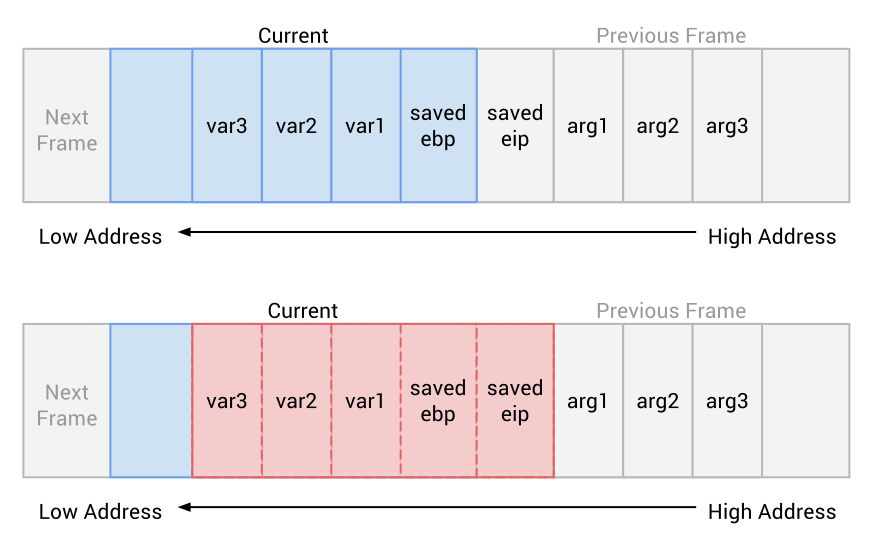
\includegraphics[width=0.95\textwidth]{img/x86-stack-layout}
    \caption{Stack Layout and Stack Overflow}
    \end{figure}
\end{frame}

\begin{frame}
    \frametitle{Disassemble bar()}
    \lstinputlisting{source/x86-disassemble-bar}
\end{frame}

\begin{frame}
    \frametitle{x86 Exploit Input}
    \begin{figure}
    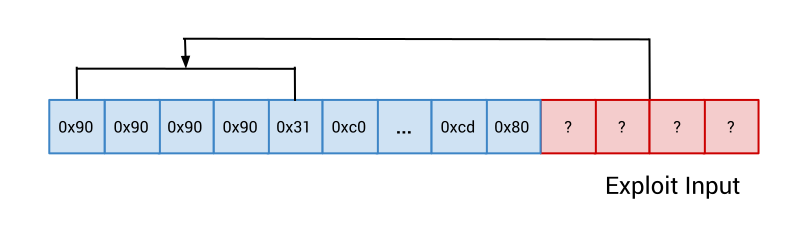
\includegraphics[width=0.95\textwidth]{img/x86-exploit-input}
    \caption{x86 Exploit Input}
    \end{figure}
\end{frame}

\section{CRAX}
\begin{frame}[c,plain,noframenumbering]
    \sectionpage
\end{frame}

\begin{frame}
    \frametitle{Manually Generate Exploit}
    \begin{figure}
    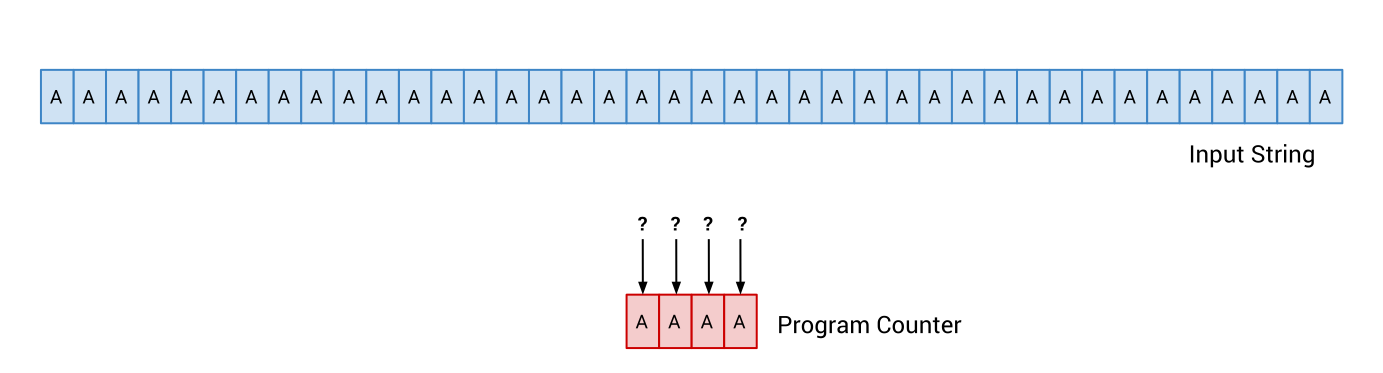
\includegraphics[width=1.0\textwidth]{img/blind-program-counter-contamination}
    \caption{Vague relationship between input string and program counter}
    \end{figure}
\end{frame}

\begin{frame}
    \frametitle{Automatically Generate Exploit}
    \begin{figure}
    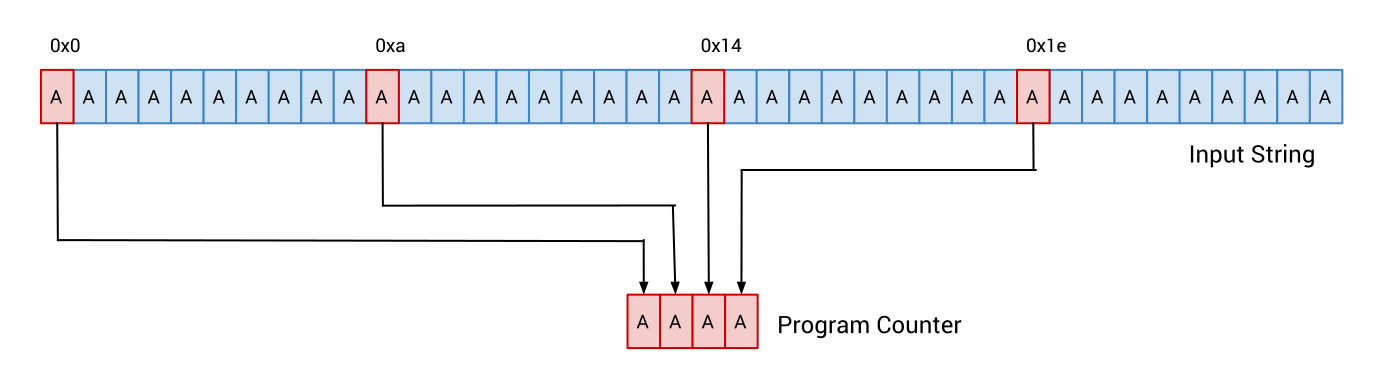
\includegraphics[width=1.0\textwidth]{img/program-counter-contamination}
    \caption{Clear relationship between input string and program counter}
    \end{figure}
    \lstinputlisting{source/symbolic-data}
\end{frame}

\begin{frame}
    \frametitle{Path Constraints}
    \lstinputlisting{source/simple-branching.c}
    \lstinputlisting{source/simple-branching-constraints}
\end{frame}

\begin{frame}
    \frametitle{Exploit Generating Process}
    \begin{figure}
    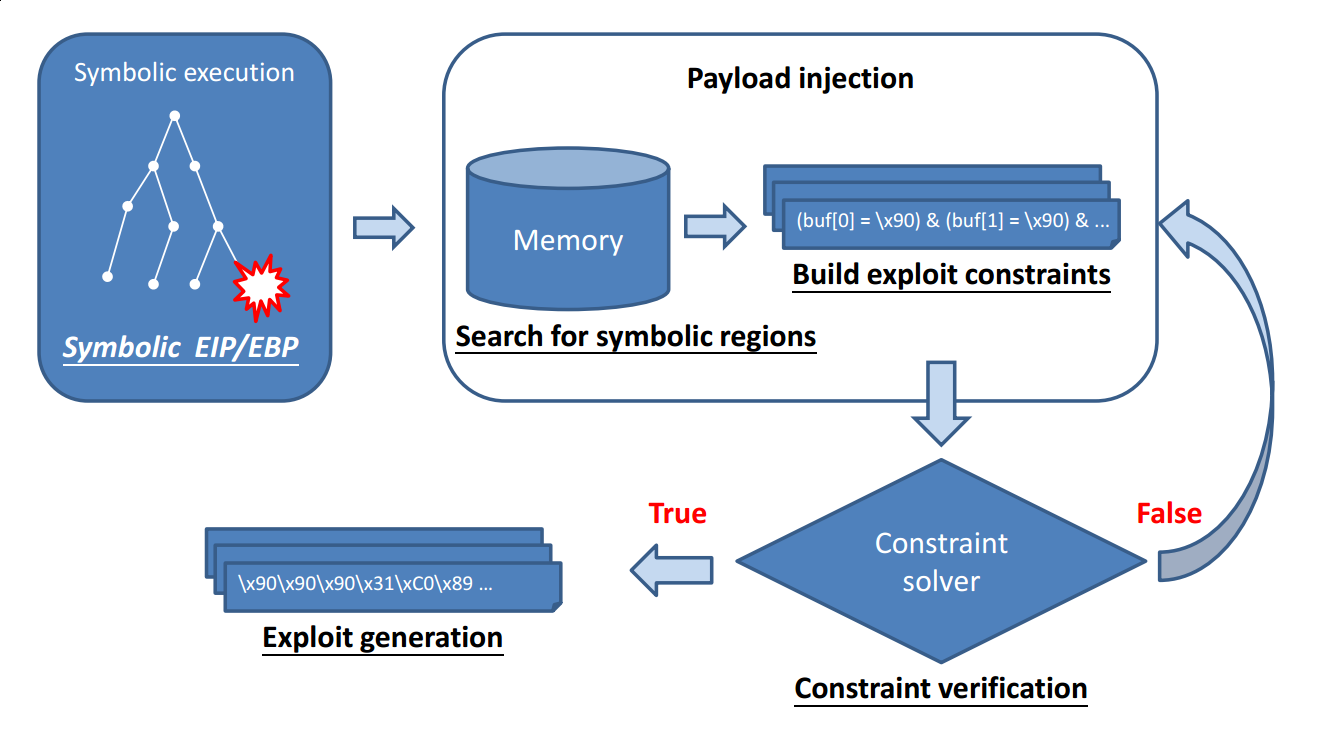
\includegraphics[width=1.0\textwidth]{img/exploit-generating-process}
    \end{figure}
\end{frame}

\section{CRAXDroid}
\begin{frame}[c,plain,noframenumbering]
    \sectionpage
\end{frame}

\begin{frame}
    \frametitle{Android System Architecture}
    \begin{figure}
    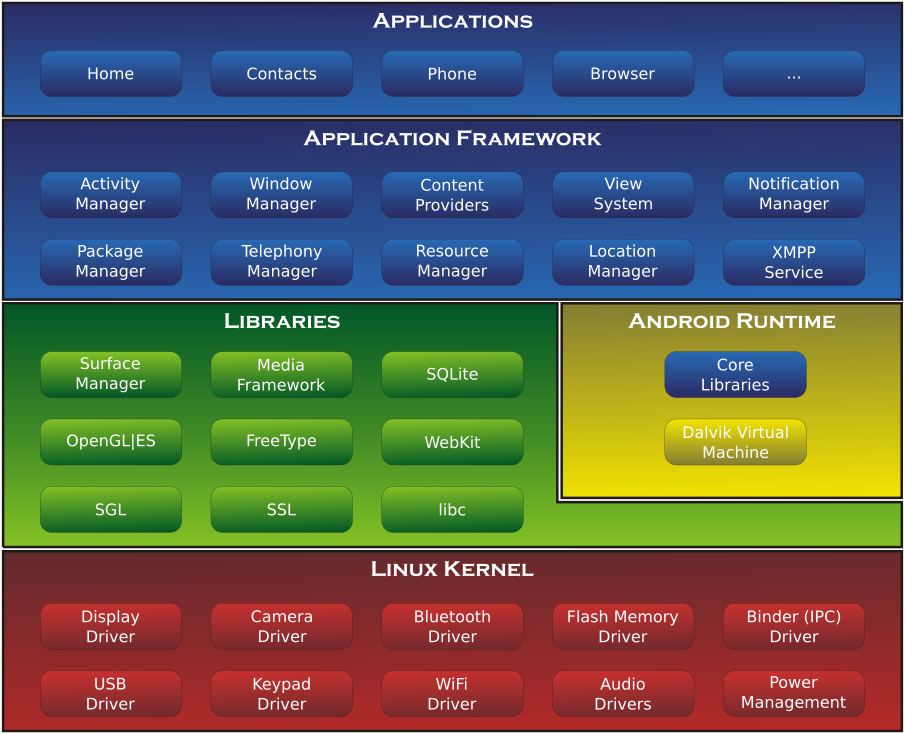
\includegraphics[width=1.0\textheight]{img/Android-System-Architecture}
    \end{figure}
\end{frame}

\begin{frame}
    \frametitle{Guinea Pig - Android x86}
    \begin{columns}
    \begin{column}{6cm}
    \begin{figure}
    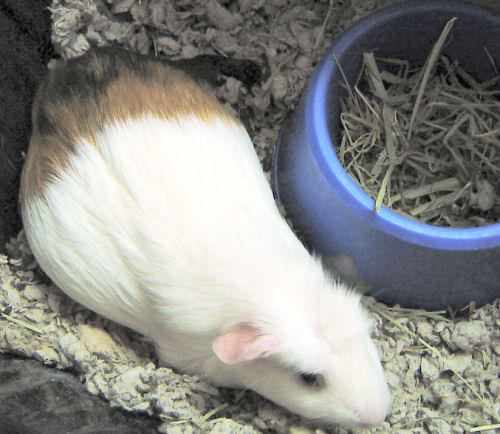
\includegraphics[width=0.8\textwidth]{img/guinea-pig}
    \end{figure}
    \end{column}
    \begin{column}{6cm}
    \begin{figure}
    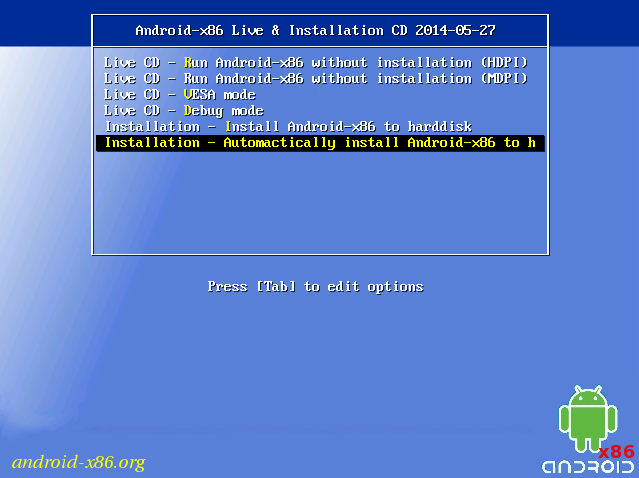
\includegraphics[width=0.9\textwidth]{img/android-x86-installation.png}
    \end{figure}
    \end{column}
    \end{columns}
\end{frame}

\begin{frame}
    \frametitle{Scenario 1 - propagate underneath Dalvik VM}
    \begin{figure}
    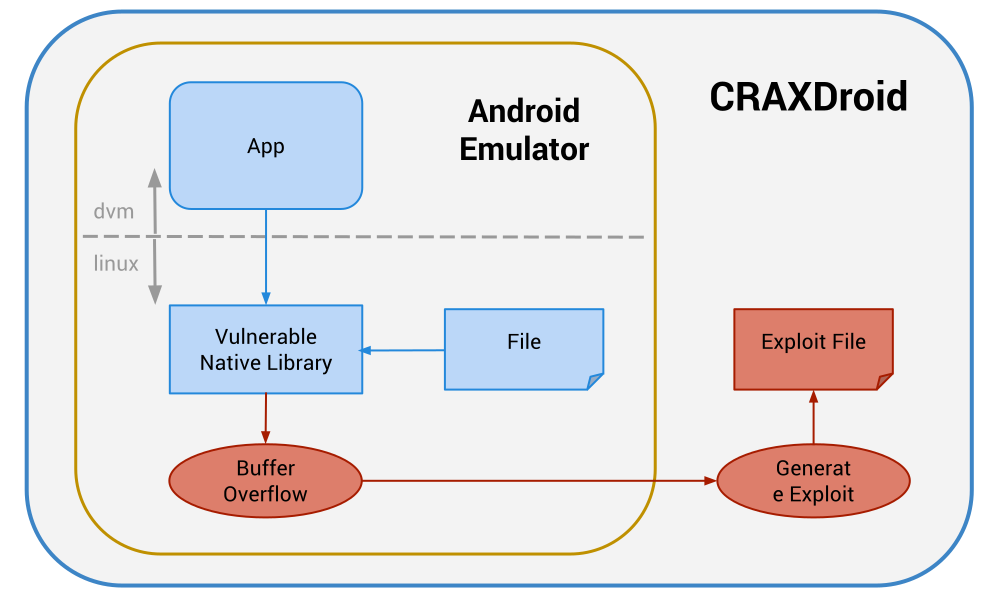
\includegraphics[width=1.0\textwidth]{img/android-exploit-scenario}
    \end{figure}
\end{frame}

\begin{frame}
    \frametitle{VulnApp1.java}
    \lstinputlisting[firstline=7,lastline=25]{source/VulnApp.java}
\end{frame}

\begin{frame}
    \frametitle{VulnApp1.c}
    \lstinputlisting{source/VulnApp-slides.c}
\end{frame}

\begin{frame}
    \frametitle{Exploit Generating Progress}
    \lstinputlisting{source/exploit-scenario1-progress-slides}
\end{frame}

\begin{frame}
    \frametitle{Generated Exploit Input}
    Exploit that will execute '/system/bin/log Exploit!'
    \lstinputlisting[numbers=none,xleftmargin=\parindent]{source/exploit-input-80e9075}
\end{frame}

\begin{frame}
    \frametitle{Exploit Verification}
    \begin{figure}
    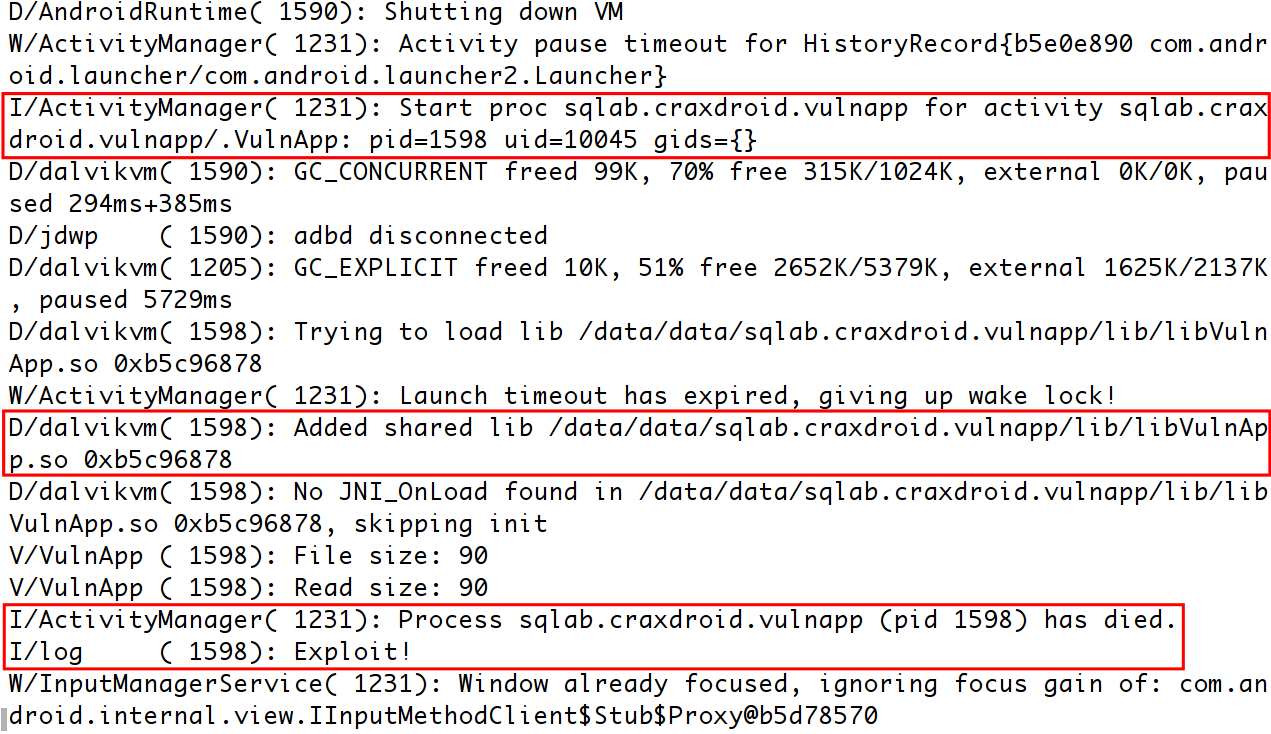
\includegraphics[width=1.0\textwidth]{img/exploit-verify}
    \end{figure}
\end{frame}

\begin{frame}
    \frametitle{Scenario 2 - propagate through Dalvik VM}
    \begin{figure}
    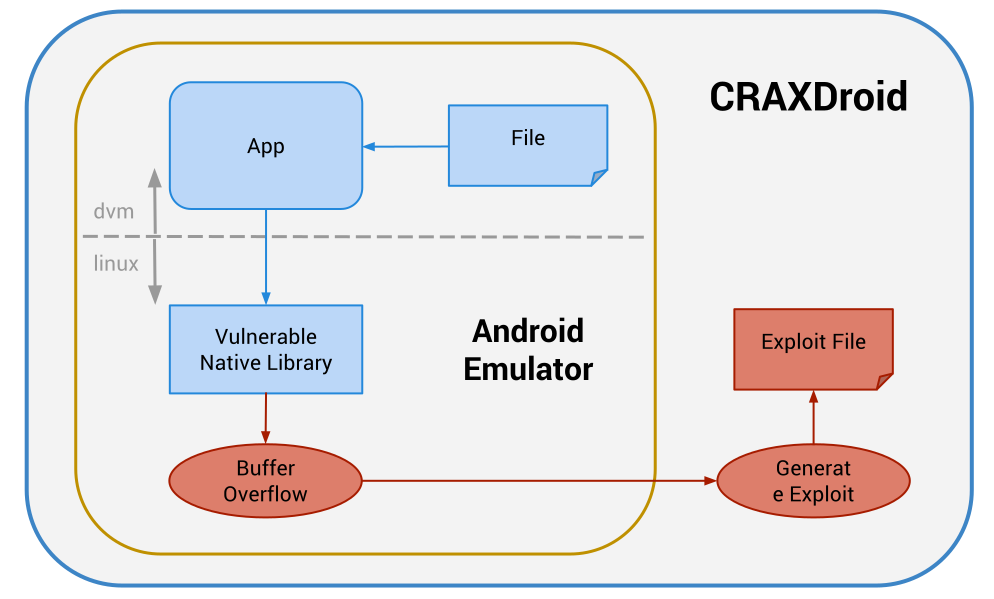
\includegraphics[width=1.0\textwidth]{img/android-exploit-scenario2}
    \end{figure}
\end{frame}

\begin{frame}
    \frametitle{VulnApp2.java}
    \lstinputlisting{source/VulnApp2-slides.java}
\end{frame}

\begin{frame}
    \frametitle{VulnApp2.c}
    \lstinputlisting[firstline=9]{source/VulnApp2.c}
\end{frame}

\begin{frame}
    \frametitle{Exploit Generating Progress}
    \lstinputlisting{source/exploit-scenario2-progress-slides}
\end{frame}

\section{CRAXDroid for ARM}
\begin{frame}[c,plain,noframenumbering]
    \sectionpage
\end{frame}

\begin{frame}
    \frametitle{Admit it}
    \begin{columns}
        \begin{column}{7.5cm}
            \begin{itemize}
                \item{You don't know how to exploit ARM}
                \item{You don't know how to run Android with QEMU}
            \end{itemize}
        \end{column}
        \begin{column}{4.5cm}
            \begin{figure}
            \reflectbox{
\includegraphics[width=0.95\linewidth]{img/me_gusta_by_rober_raik-d4clrpu.png}}
            \end{figure}
        \end{column}
    \end{columns}
\end{frame}

\section{Exploit programs on ARM}
\begin{frame}[c,plain,noframenumbering]
    \sectionpage
\end{frame}

\begin{frame}
    \frametitle{Smashing Raspberry Pi}
    \begin{figure}
    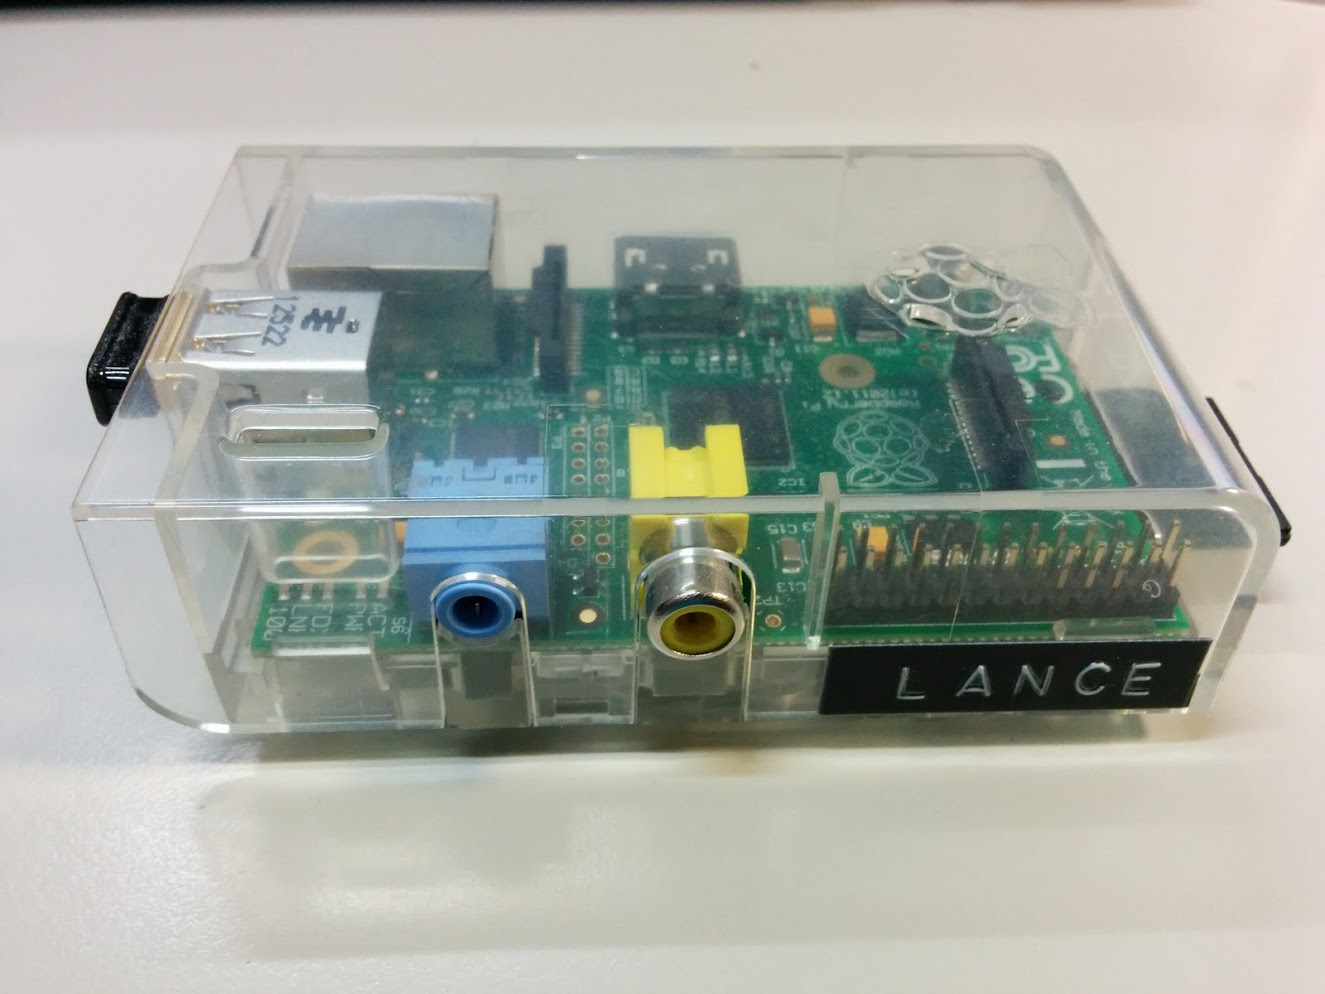
\includegraphics[width=0.9\textwidth]{img/rpi.jpg}
    \end{figure}
\end{frame}

\begin{frame}
    \frametitle{Again the Simple Vunerable Program}
    \lstinputlisting{source/simple-vulnerable-program.c}
\end{frame}

\begin{frame}
    \frametitle{CRASHED!}
    \begin{figure}
    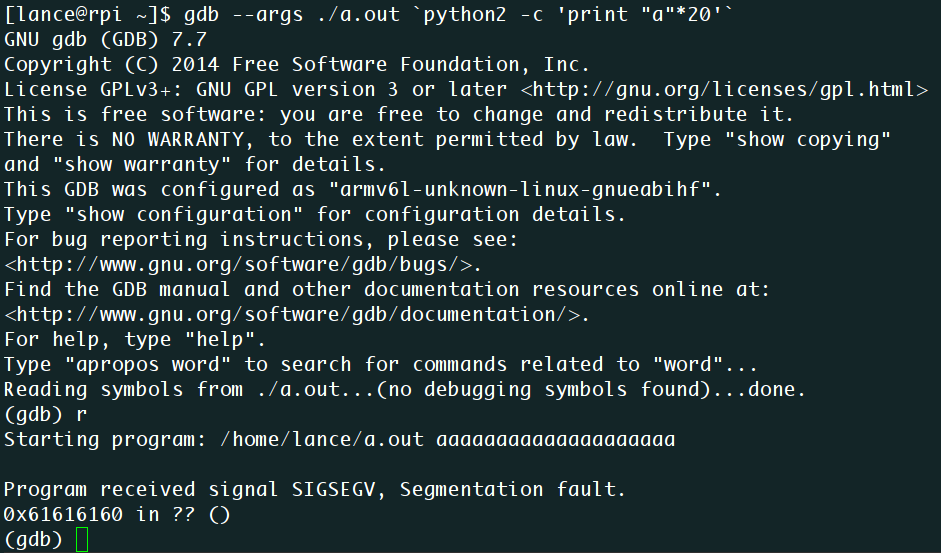
\includegraphics[width=0.95\textwidth]{img/arm-crash}
    \end{figure}
\end{frame}

\begin{frame}
    \frametitle{ARM Registers}
    \begin{itemize}
        \item{r15 - program counter}
        \item{r14 - link register}
        \item{r13 - stack pointer}
        \item{r12}
        \item{r4 to r11 - local variables}
        \item{r0 to r3 - subroutine arguments}
    \end{itemize}
\end{frame}

\begin{frame}
    \frametitle{ARM Calling Convention}
    \begin{figure}
    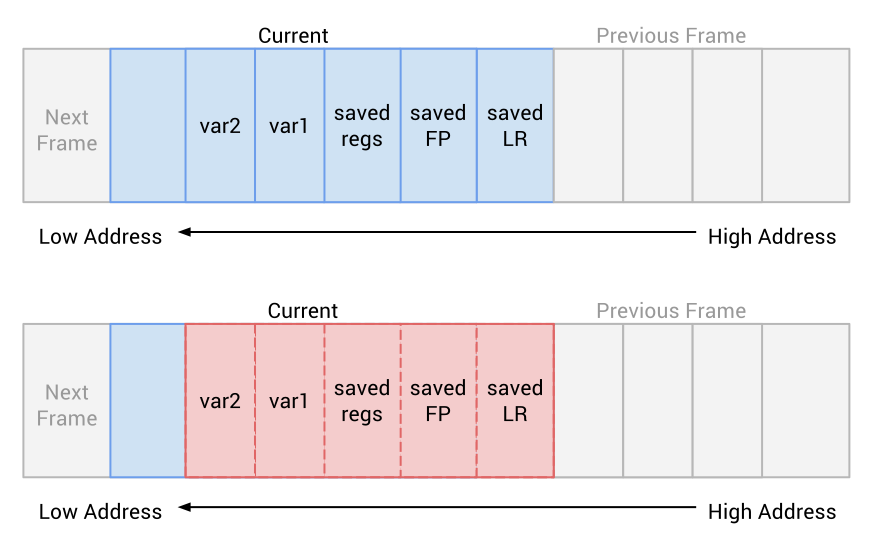
\includegraphics[width=0.95\textwidth]{img/arm-calling-convention}
    \caption{ARM Calling Convention}
    \end{figure}
\end{frame}

\begin{frame}
    \frametitle{Disassemble bar()}
    \lstinputlisting{source/arm-disassemble-bar}
\end{frame}

\section{CRAX for ARM}
\begin{frame}[c,plain,noframenumbering]
    \sectionpage
\end{frame}

\begin{frame}
    \frametitle{Reimplement CRAX for ARM Support}
    \begin{figure}
    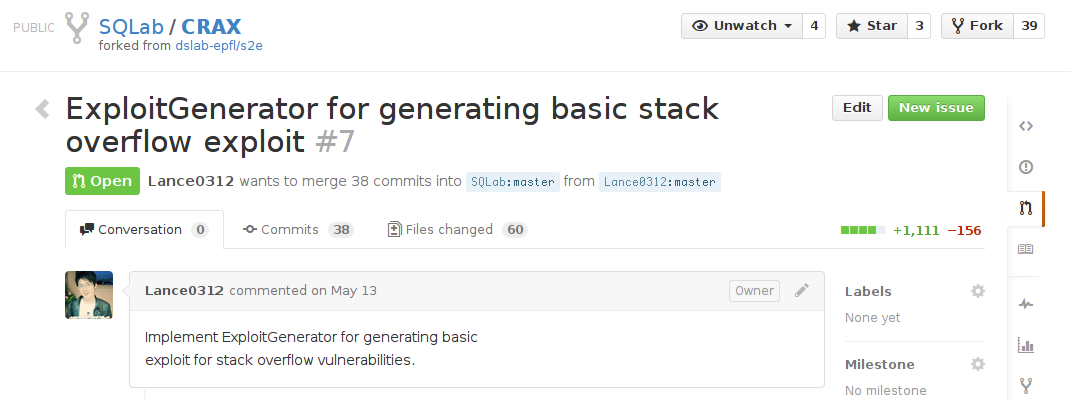
\includegraphics[width=1.0\textwidth]{img/crax-pull-request.png}
    \caption{CRAX Pull Request \#7}
    \end{figure}
\end{frame}

\begin{frame}
    \frametitle{Raspbian}
    \begin{figure}
    
\includegraphics[width=1.0\textwidth]{img/raspbian_logo.png}
    \end{figure}
\end{frame}

\begin{frame}
    \frametitle{Yet Again the Simple Vunerable Program}
    \lstinputlisting{source/simple-vulnerable-program.c}
\end{frame}

\begin{frame}
    \frametitle{Exploit Generating Progress}
    \lstinputlisting{source/raspbian-exploit-bof-progress}
\end{frame}

\begin{frame}
    \frametitle{aeon - CVE-2005-1019}
    \lstinputlisting{source/lib_aeon.c}
\end{frame}

\begin{frame}
    \frametitle{Exploit Generating Progress - aeon}
    \lstinputlisting{source/raspbian-exploit-aeon-progress}
\end{frame}

\begin{frame}
    \frametitle{htget - CVE-2004-0852}
    \lstinputlisting{source/htget.c}
\end{frame}

\begin{frame}
    \frametitle{Exploit Generating Progress - htget}
    \lstinputlisting{source/raspbian-exploit-htget-progress}
\end{frame}

\section{Conclusions}
\begin{frame}[c,plain,noframenumbering]
    \sectionpage
\end{frame}

\begin{frame}
    \frametitle{My Contributions}
    \begin{itemize}
        \item{Proved that Android is a potential victim of CRAX}
        \item{First step to ARM exploit generating for CRAX}
    \end{itemize}
\end{frame}

\begin{frame}
    \frametitle{Future Works}
    \begin{itemize}
        \item{Emulating Android ARM with pure QEMU}
        \item{Real Exploit For ARM (x86 as well)}
        \item{Testing on Various ARM architecures}
        \item{Improve S$^{2}$E ARM supporting}
    \end{itemize}
\end{frame}

\end{document}

% End of file
